\setlength{\columnsep}{3pt}
\begin{flushleft}
	\bigskip
	\begin{itemize}
		\begin{itemize}
			\item DHCP stands for \textbf{D}ynamic \textbf{H}ost \textbf{C}ontrol \textbf{P}rotocol.
			\item Using DHCP server, systems can obtain IP address automatically at boot time.
			\item If a DHCP server is not available, the system uses a static configuration from a local configuration file.
			\item Only one address can be assigned per NIC card with DHCP. 
			\item In your home, router acts like a DHCP server and assign IP address to all connected device.
			\begin{figure}[h!]
				\centering
				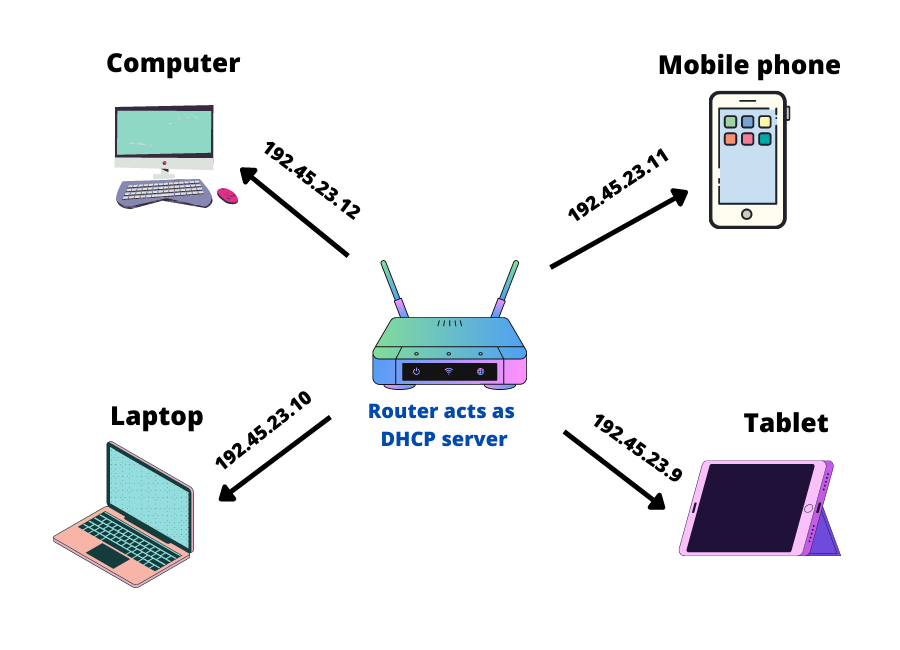
\includegraphics[scale=0.5]{content/chapter14/images/dhcp.png}
				\caption{DHCP server}
				\label{fig:severity6}
			\end{figure}			
		\end{itemize}
	\end{itemize}
	
 \end{flushleft}
\newpage


